\documentclass[11pt, a4paper]{article}

\usepackage{CJK}
\usepackage{caption}
\usepackage{graphicx, subfig}
\usepackage{booktabs}
\usepackage{geometry}
\geometry{left=2.5cm, right=2.5cm, top=2.5cm, bottom=2.5cm}
\usepackage{amsmath}
\usepackage{mathrsfs}
\usepackage{lipsum}
\usepackage{amsfonts}
\usepackage{indentfirst}
\usepackage{url}
\usepackage{amssymb}
\usepackage{algorithm}
\usepackage{algorithmicx}
\usepackage{algpseudocode}
\usepackage{enumerate}
\newtheorem{myDef}{Definition}
\newtheorem{myTheo}{Theorem}

\usepackage{listings}
\usepackage{color} %red, green, blue, yellow, cyan, magenta, black, white
\definecolor{mygreen}{RGB}{28,172,0} % color values Red, Green, Blue
\definecolor{mylilas}{RGB}{170,55,241}

\usepackage{pythonhighlight}
\usepackage{listings}
\usepackage{color} %red, green, blue, yellow, cyan, magenta, black, white

% \definecolor{mygreen}{rgb}{0,0.6,0}
\definecolor{mygray}{rgb}{0.5,0.5,0.5}
\definecolor{mymauve}{rgb}{0.58,0,0.82}
\lstset{
    backgroundcolor=\color{white},   % choose the background color
    basicstyle=\footnotesize\ttfamily,        % size of fonts used for the code
    columns=fullflexible,
    breaklines=true,                 % automatic line breaking only at whitespace
    captionpos=b,                    % sets the caption-position to bottom
    tabsize=4,
    commentstyle=\color{mygreen},    % comment style
    escapeinside={\%*}{*)},          % if you want to add LaTeX within your code
    keywordstyle=\color{blue},       % keyword style
    stringstyle=\color{mymauve}\ttfamily,     % string literal style
    frame=single,
    rulesepcolor=\color{red!20!green!20!blue!20},
    % identifierstyle=\color{red},
    language=Python,
}


\floatname{algorithm}{�㷨}
\renewcommand{\algorithmicrequire}{\textbf{����:}}
\renewcommand{\algorithmicensure}{\textbf{���:}}


\numberwithin{equation}{section}

\begin{document}
\begin{CJK*}{GBK}{song}  % song kai li hei
\title{Project 3: Finite Element Method to Solve Partial Differential Equations with Boundary Conditions }
\author{Ji, Jingwei ~~5141209098~~~No.~10 }
% \date{}
\maketitle


\section{The problem}\label{sec:intro}
    Consider the following one-dimensional elliptic equations with boundary condition��
    \begin{equation}\label{eq:equestion}
        \left\{
            \begin{aligned}
                 -\left(p(x)u'(x) \right)' + u(x) = f(x) ,~~~0<x<1,  \\
                u(0)=0,~~p(1)u'(1)+u(1)=\beta
            \end{aligned}
        \right.
    \end{equation}
    where $p(x) = 1+x^2$.

    In this report, I set $u(x)=\sin(x)$. Thus the following are subsequently determined:
    \begin{eqnarray}
      f(x) &=& 2 \sin x - 2x\cos x + x^2 \sin x \\
      \beta &=& 2 \cos(1) + \sin(1)
    \end{eqnarray}


\section{The virtual work statement equivalent to \ref{eq:equestion}}
    The space of admissible functions is $V=\{v| v \text{ is sufficiently smooth} on [0,1], v(0)=0  \} $��

    It is to find $u \in V$, such that $\forall v \in V$:
    \begin{equation}
        \int_{0}^{1} \left [ -\left(p u' \right)' + u \right] v dx = \int_{0}^{1} fv dx
    \end{equation}
    After a bit calculus, the above turns to
    $$
    \int_{0}^{1} \left [ pu'v' + uv \right ] dx + u(1)v(1) = \int_{0}^{1} fv dx + \beta v(1)
    $$

    Define $a(u, v) \triangleq \int_{0}^{1} \left [ pu'v' + uv \right ] dx + u(1)v(1)$ and $ F(v) \triangleq \int_{0}^{1} fv dx + \beta v(1) $. Now solving \ref{eq:equestion} is equivalent to finding  $u \in V$, such that
     \begin{equation}\label{eq:Galerkin}
       a(u, v)=F(v), ~~\forall v \in V
     \end{equation}


\section{The construction of finite element method}
\subsection{A general case}
    $V$ has infinite degrees of freedom, which is impossible to solve. Consider the  discretized space, $U_h = \{v | v \in C[0,1]; v | e_k \in P_1 (e_k), 1 \leq k \leq N   \}$, where $e_k$ is a partition, $e_k = [x_{k-1}, x_k]$, and $P_1$ is polynomials of order one. Denote by $h_k = x_k - x_{k-1} $ the length of each interval, and define $h= \max_{1 \leq k \leq N} h_k $. Clearly $U_h \subseteq V$.

    Denote by
    $$
    \phi_0 = \left\{
            \begin{aligned}
                 1  - \frac{1}{h_1} (x-x_0) &,~~~x_0=0 \leq x \leq x_1,  \\
                0&,~~~\text{else}
            \end{aligned}
        \right.
    $$
    $$
    \phi_i = \left\{
            \begin{aligned}
                \frac{1}{h_i} (x-x_{i-1}) &,~~~x_{i-1} \leq x \leq x_i,  \\
                -\frac{1}{h_{i+1}}(x-x_{i+1}) &,~~~ x_i \leq   x  \leq x_{i+1}   \\
                0&, ~~~ \text{else}
            \end{aligned}
        \right.
    $$
    $i=1,2,...,N-1$.
    $$
    \phi_N = \left\{
        \begin{aligned}
            \frac{1}{h_N}(x-x_{N-1}) &,~~~x_{N-1} \leq x \leq x_N=1 \\
            0&, ~~~\text{else}
        \end{aligned}
        \right.
    $$
    It can be shown that $\phi_i,i=0,1,...,N$ is a set of basis of $U_h$. Thus $\forall v \in U_h$, $v=\sum_{i=0}^{N} v_i \phi_i$.

    To further incorporate into the type I boundary condition, we constrain $U_h$ to $V_h = \{v | v \in C[0,1]; v | e_k \in P_1 (e_k), 1 \leq k \leq N  ; v(0) = 0 \}$. Clearly it has freedom of $N$, and $\forall v \in V_h$, $v=\sum_{i=1}^{N} v_i \phi_i$.

    The idea of finite element method is to find a $u_h = \sum_{i=1}^{N} u_i \phi_i $ in $V_h$ to approximate the real solution $u$. And note that \ref{eq:Galerkin} turns to
    \begin{equation}\label{eq:Galerkin_u}
        a(u_h, v) = F(v),~~~\forall v \in V_h
    \end{equation}
    So it suffices to find $u_h \in V_h$, such that
    $$
        a(u_h, \phi_i) = F(\phi_i),~~~i=1,2,...,N
    $$
    Substituting $u_h = \sum_{i=1}^{N} u_i \phi_i $ into above we have
    $$
        \sum_{i=1}^{N} a(\phi_i, \phi_j) u_i = F(\phi_j), ~~~j=1,2,...,N
    $$
    Denote by $ A = [a(\phi_i, \phi_j )]_{ij}$, $\overrightarrow{u}=\begin{bmatrix}
                                                                      u_1 \\
                                                                      u_2 \\
                                                                      \vdots \\
                                                                      u_N
                                                                    \end{bmatrix}$, $\overrightarrow{F} =\begin{bmatrix}
                                                     F(\phi_1) \\
                                                     F(\phi_2) \\
                                                     \vdots \\
                                                     F(\phi_N)
                                                   \end{bmatrix}$, and then we can write
    \begin{equation}
      A \overrightarrow{u} = \overrightarrow{F}
    \end{equation}
\subsection{A computable form}
    Now consider how to express the integration in $a(u,v)$ and $F(v)$ in a computable manner, where $u,v\in V_h$, meaning $u(x) = \sum_{k=1}^{N} u_k \phi_k(x)$, $v(x) = \sum_{k=1}^{N} v_k \phi_k(x) $.  Define $N_k(x) = \frac{x_k-x}{h_k}$, $M_k(x) = \frac{x-x_{k-1}}{h_k}$, then $u(x) = u_{k-1} N_k(x) + u_k M_k (x)$, $v(x) = v_{k-1} N_k(x) + v_k M_k (x)$ respectively on $e_k$.

    \begin{eqnarray*}
      a(u,v) & \triangleq &  \int_{0}^{1} \left [ pu'v' + uv \right ] dx + u(1)v(1)  \\
      &=&  \sum_{k=1}^{N} \left[ \int_{e_k}^{} pu'v'+un dx \right] + u(1)v(1) \\
      & \triangleq & \sum_{k=1}^{N} a_k(u,v)
    \end{eqnarray*}
    where
    $$
    a_k(u,v) = \int_{e_k} pu'v' + uvdx, ~~~1 \leq k \leq N-1
    $$
    $$
    a_N(u,v) = \int_{e_N} pu'v'+uvdx + u(1)v(1)
    $$

    For $1 \leq k \leq N-1$,
    \begin{eqnarray*}
    % \nonumber % Remove numbering (before each equation)
      a_k(u,v) &=& \left [ \int_{e_k}  p(x) N_k'(x)^2 + N_k(x)^2  dx  \right] u_{k-1} v_{k-1} \\
       &+& \left [ \int_{e_k}  p(x) N_k'(x) M_k'(x) + N_k(x) M_k(x)  dx  \right] u_{k-1} v_k \\
       &+& \left [ \int_{e_k}    p(x) N_k'(x) M_k'(x) + N_k(x) M_k(x)  dx   \right] u_k v_{k-1} \\
       &+& \left [ \int_{e_k}   p(x) M_k'(x)^2 + M_k(x)^2  dx  \right] u_k v_k  \\
       &=& \left[ \frac{\frac{2}{3} x_k^3 - \frac{2}{3} x_{k-1}^3 + x_kx_{k-1}^2 - x_k^2x_{k-1} +x_k - x_{k-1} }{(x_k - x_{k-1})^2}   \right]   u_{k-1} v_{k-1}  \\
       &+& \left[ \frac{ -\frac{1}{6} x_k^3 + \frac{1}{6} x_{k-1}^3 -x_k +x_{k-1} -\frac{1}{2} x_{k-1}x_k^2 + \frac{1}{2} x_k x_{k-1}^2  }{(x_k - x_{k-1})^2}   \right ] u_{k-1} v_k \\
       &+& \left[ \frac{ -\frac{1}{6}x_k^3 + \frac{1}{6} x_{k-1}^3 - x_k + x_{k-1} + \frac{1}{2} x_k x_{k-1}^2 - \frac{1}{2} x_{k-1} x_k^2   }{(x_k - x_{k-1})^2}   \right ] u_k v_{k-1} \\
       &+& \left[  \frac{ \frac{2}{3} x_k^3 - \frac{2}{3} x_{k-1}^3 + x_k - x_{k-1} + x_{k-1}^2 x_k - x_{k-1} x_k^2  }{ (x_k - x_{k-1})^2 }  \right ]  u_k v_k \\
    \end{eqnarray*}
    % \left [ \frac{x_k^2 + 1 }{x_k - x_{k-1}} - \frac{1}{3} x_k - \frac{2}{3} x_{k-1}   \right ]  u_{k-1} v_{k-1} \\
    %   &+& \left [ - \frac{1}{6} x_k + \frac{7}{6} x_{k-1} - \frac{x_{k-1}x_k + 1}{x_k - x_{k-1}}    \right ] u_{k-1} v_k  \\
    %   &+& \left [  - \frac{1}{6} x_k + \frac{7}{6} x_{k-1} - \frac{x_{k-1}x_k + 1}{x_k - x_{k-1}}     \right ] u_k v_{k-1} \\
    %   &+& \left [  \frac{x_{k-1}^2+1}{x_k - x_{k-1} } + \frac{2}{3} x_k - \frac{5}{3} x_{k-1}    \right ] u_k v_k



    For $ k = N$,
    \begin{eqnarray*}
    % \nonumber % Remove numbering (before each equation)
      a_N(u,v) &=&  \left[ \frac{\frac{2}{3} x_N^3 - \frac{2}{3} x_{N-1}^3 + x_N x_{N-1}^2 - x_N^2 x_{N-1} +x_N - x_{N-1} }{(x_N - x_{N-1})^2}   \right]   u_{N-1} v_{N-1}  \\
       &+& \left[ \frac{ -\frac{1}{6} x_N^3 + \frac{1}{6} x_{N-1}^3 -x_N +x_{N-1} -\frac{1}{2} x_{N-1}x_N^2 + \frac{1}{2} x_N x_{N-1}^2  }{(x_N - x_{N-1})^2}   \right ] u_{N-1} v_N \\
       &+& \left[ \frac{ -\frac{1}{6}x_N^3 + \frac{1}{6} x_{N-1}^3 - x_N + x_{N-1} + \frac{1}{2} x_N x_{N-1}^2 - \frac{1}{2} x_{N-1} x_N^2   }{(x_N - x_{N-1})^2}   \right ] u_N v_{N-1} \\
       &+& \left[  \frac{ \frac{2}{3} x_N^3 - \frac{2}{3} x_{N-1}^3 + x_N - x_{N-1} + x_{N-1}^2 x_N - x_{N-1} x_N^2  }{ (x_N - x_{N-1})^2 }  + 1 \right ]  u_N v_N
    \end{eqnarray*}

    Similarly, for $F(v)$,
    \begin{eqnarray*}
    % \nonumber % Remove numbering (before each equation)
      F(v) &\triangleq &  \int_{0}^{1} fv dx + \beta v(1) \\
       % &=&  \int_{0}^{1} \left[  2 \sin x - 2x\cos x + x^2 \sin x  \right] v(x) dx + \left(2 \cos(1) + \sin(1)\right) v(1)  \\
       &=& \sum_{k=1}^{N} \int_{e_k}^{} fv dx + \beta v(1) \\
       &\triangleq & \sum_{k=1}^{N} F_k(v)
    \end{eqnarray*}

    For $1 \leq k \leq N-1$,
    \begin{eqnarray*}
    % \nonumber % Remove numbering (before each equation)
      F_k(v) &=& \left [ \int_{x_{k-1}}^{x_k} f(x) N_k(x) dx \right] v_{k-1} + \left [  \int_{x_{k-1}}^{x_k} f(x) M_k(x) dx \right ] v_k  \\
       &=& \left [
       \frac{x_k}{x_k - x_{k-1}} (- 2 \cos x - x^2 \cos x  ) |_{x=x_{k-1}}^{x=x_k}  - \frac{1}{x_k - x_{k-1} } (x^2 \sin x - x^3 \cos x)|_{x=x_{k-1}}^{x=x_k}  \right ]   v_{k-1}   \\
       &+& \left [  - \frac{x_{k-1}}{x_k - x_{k-1}}( -2 \cos x - x^2 \cos x  ) |_{x=x_{k-1}}^{x=x_k}  +  \frac{1}{x_k - x_{k-1}} (x^2 \sin x - x^3 \cos x)|_{x=x_{k-1}}^{x=x_k}     \right ]  v_k
    \end{eqnarray*}

    For $ k = N$,
    \begin{eqnarray*}
      F_N(v) &=& \int_{x_{N-1}}^{x_N} fv dx  + \beta v(1) \\
       &=& \left [
       \frac{x_N}{x_N - x_{N-1}} (- 2 \cos x - x^2 \cos x  ) |_{x=x_{N-1}}^{x=x_N}  - \frac{1}{x_N - x_{N-1} } (x^2 \sin x - x^3 \cos x)|_{x=x_{N-1}}^{x=x_N}  \right ]   v_{N-1}   \\
       &+& \left [  - \frac{x_{N-1}}{x_N - x_{N-1}}( -2 \cos x - x^2 \cos x  ) |_{x=x_{N-1}}^{x=x_N}  +  \frac{1}{x_N - x_{N-1}} (x^2 \sin x - x^3 \cos x)|_{x=x_{N-1}}^{x=x_N}  + \beta  \right ]  v_N
    \end{eqnarray*}

    The above expressions provide a computable way to specify the matrix $A$ without computing integration numerically. For implementation codes, please see the appendix.

\section{Numerical experiments}
    I implement this specific finite element method using Python. Figure \ref{fig:n10} to \ref{fig:n10000} show the computed solution under different partition size. "Method 1" refers to evenly discretization of the x axis. Table \ref{tab:error} exhibits the relative error \footnote{The relative error here refers to $\max_i |\frac{\widetilde{ u(x_i)} - u(x_i)}{u(x_i)}|$} under different $N$. Clearly we find that the finite element method has a nice precision, even when $N$ is rather small. And the max relative error decreases as $N$ increases, except at the case when $N=10000$. 
    
    \begin{table}[htbp]
      \centering
      \caption{Evenly discretized}
        \begin{tabular}{cc}
        \toprule
        $N$   & Max relative error \\
        \midrule
        10    & 8.93E-05 \\
        100   & 8.93E-07 \\
        1000  & 8.56E-09 \\
        10000 & 2.76E-07 \\
        \bottomrule
        \end{tabular}%
      \label{tab:error}%
    \end{table}%


\begin{figure}
  \centering
  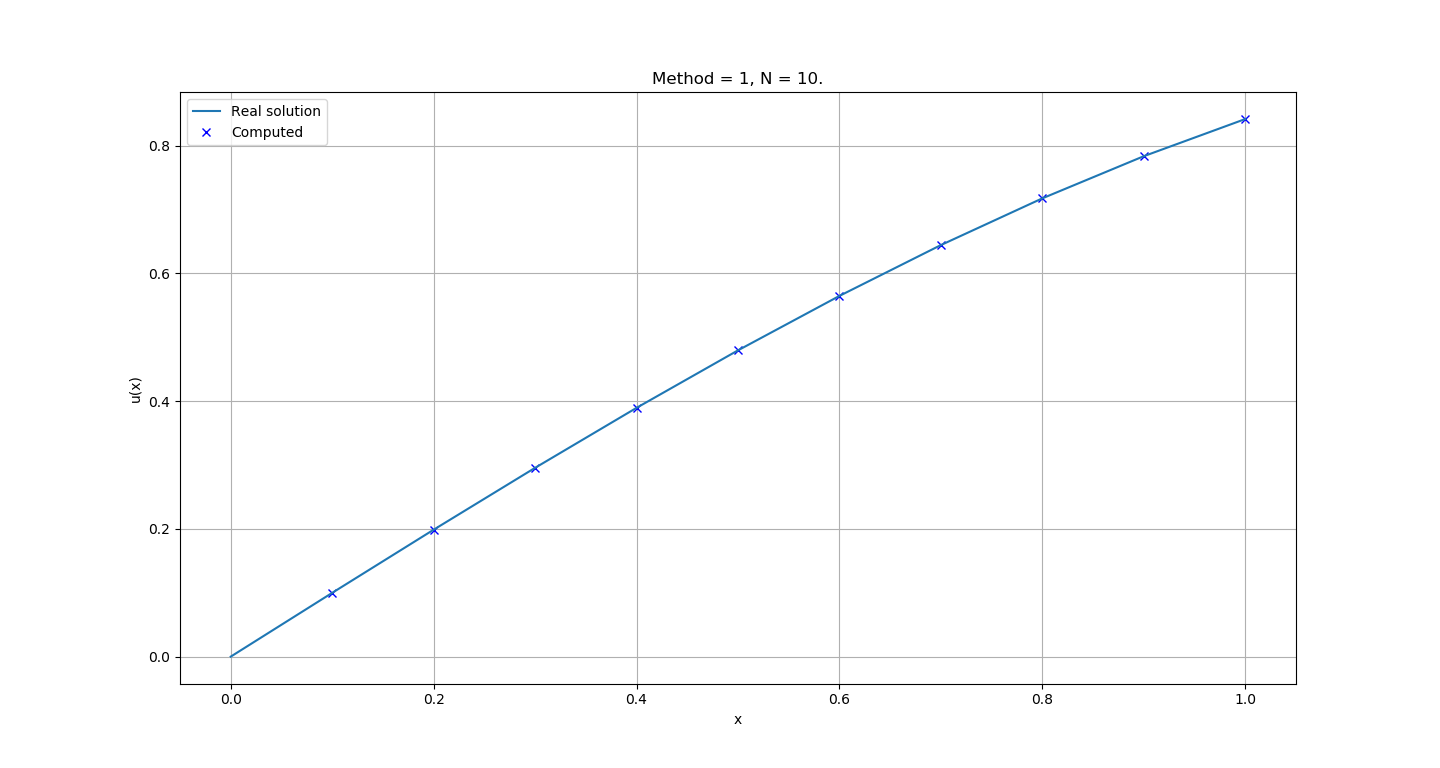
\includegraphics[width=14cm]{Figures/n10.png}
  \caption{Computed solution}\label{fig:n10}
\end{figure}

\begin{figure}
  \centering
  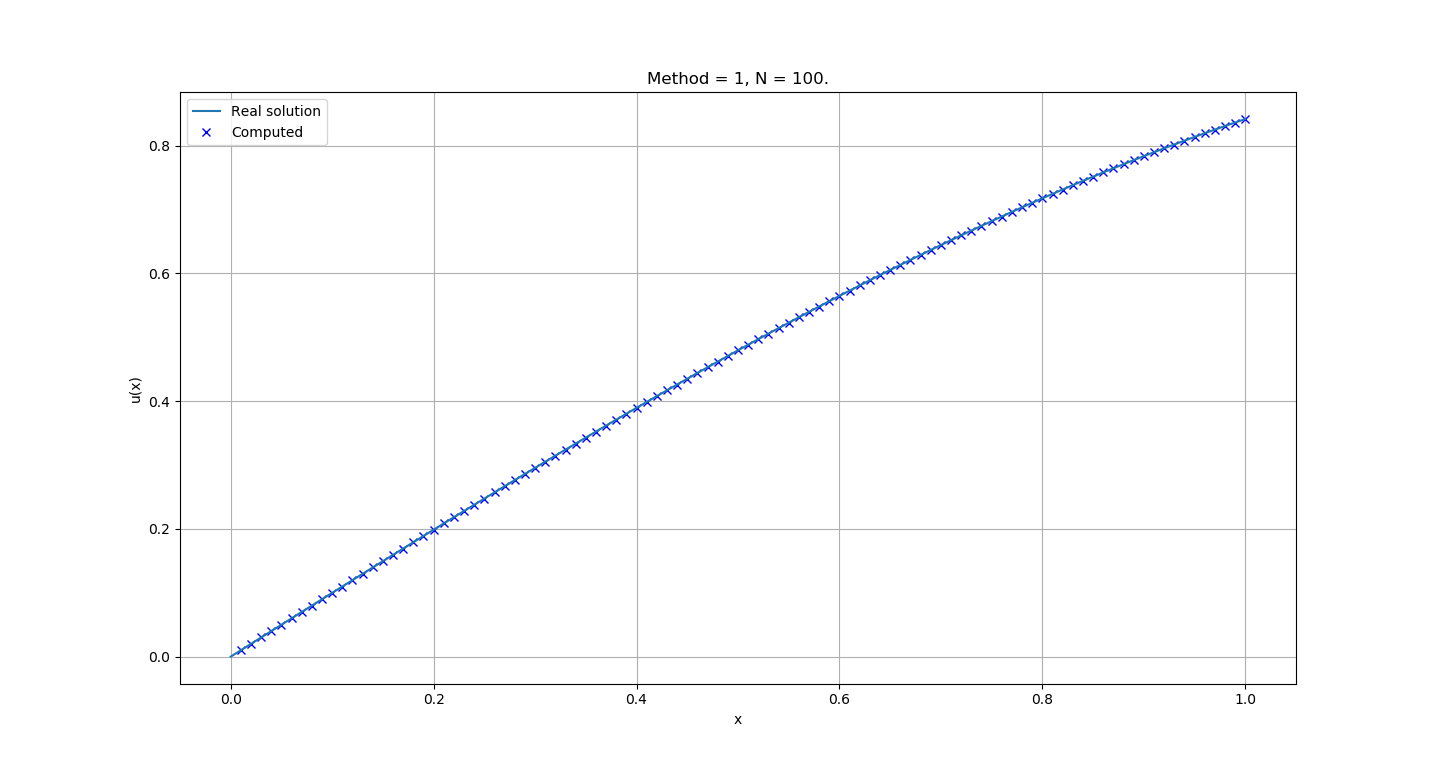
\includegraphics[width=14cm]{Figures/n100.png}
  \caption{Computed solution}\label{fig:n100}
\end{figure}

\begin{figure}
  \centering
  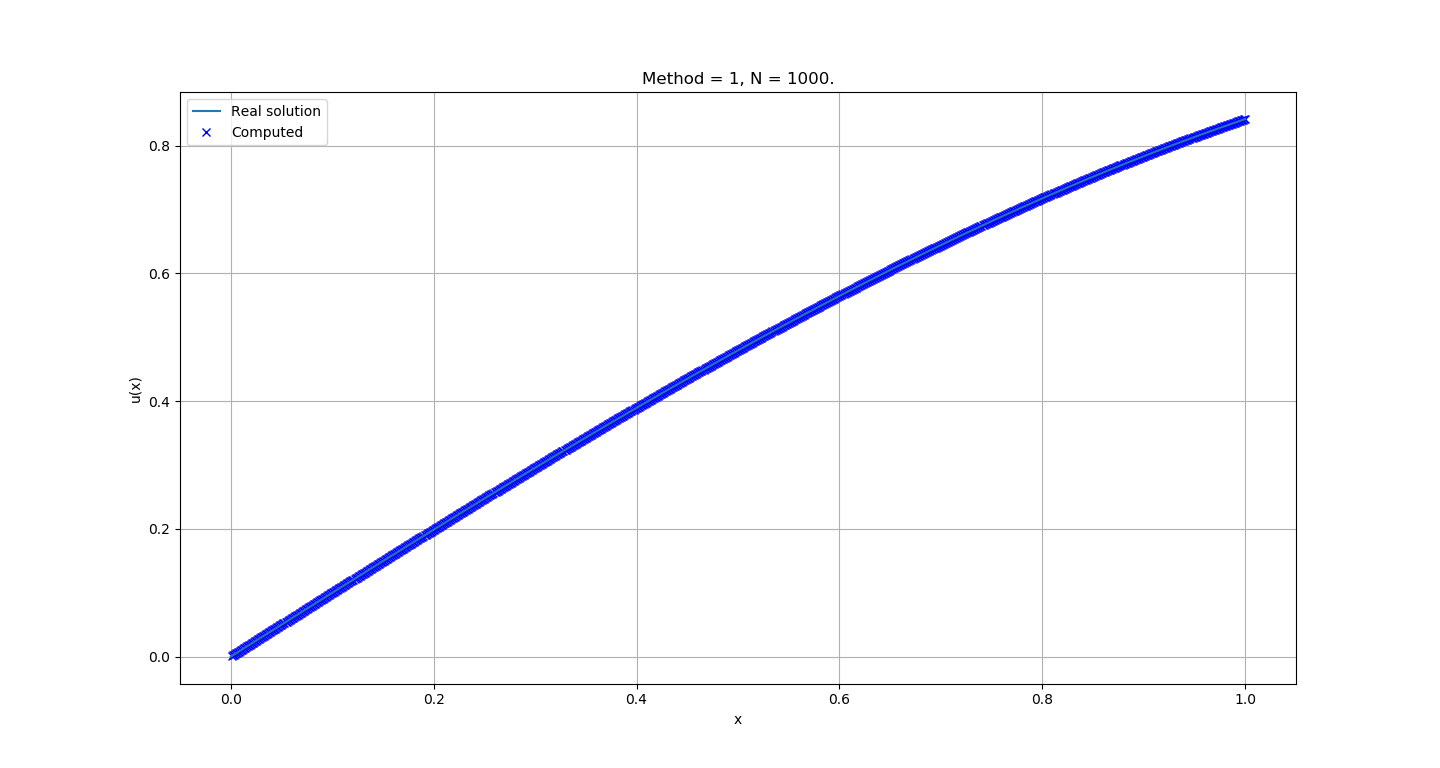
\includegraphics[width=14cm]{Figures/n1000.png}
  \caption{Computed solution}\label{fig:n1000}
\end{figure}

\begin{figure}
  \centering
  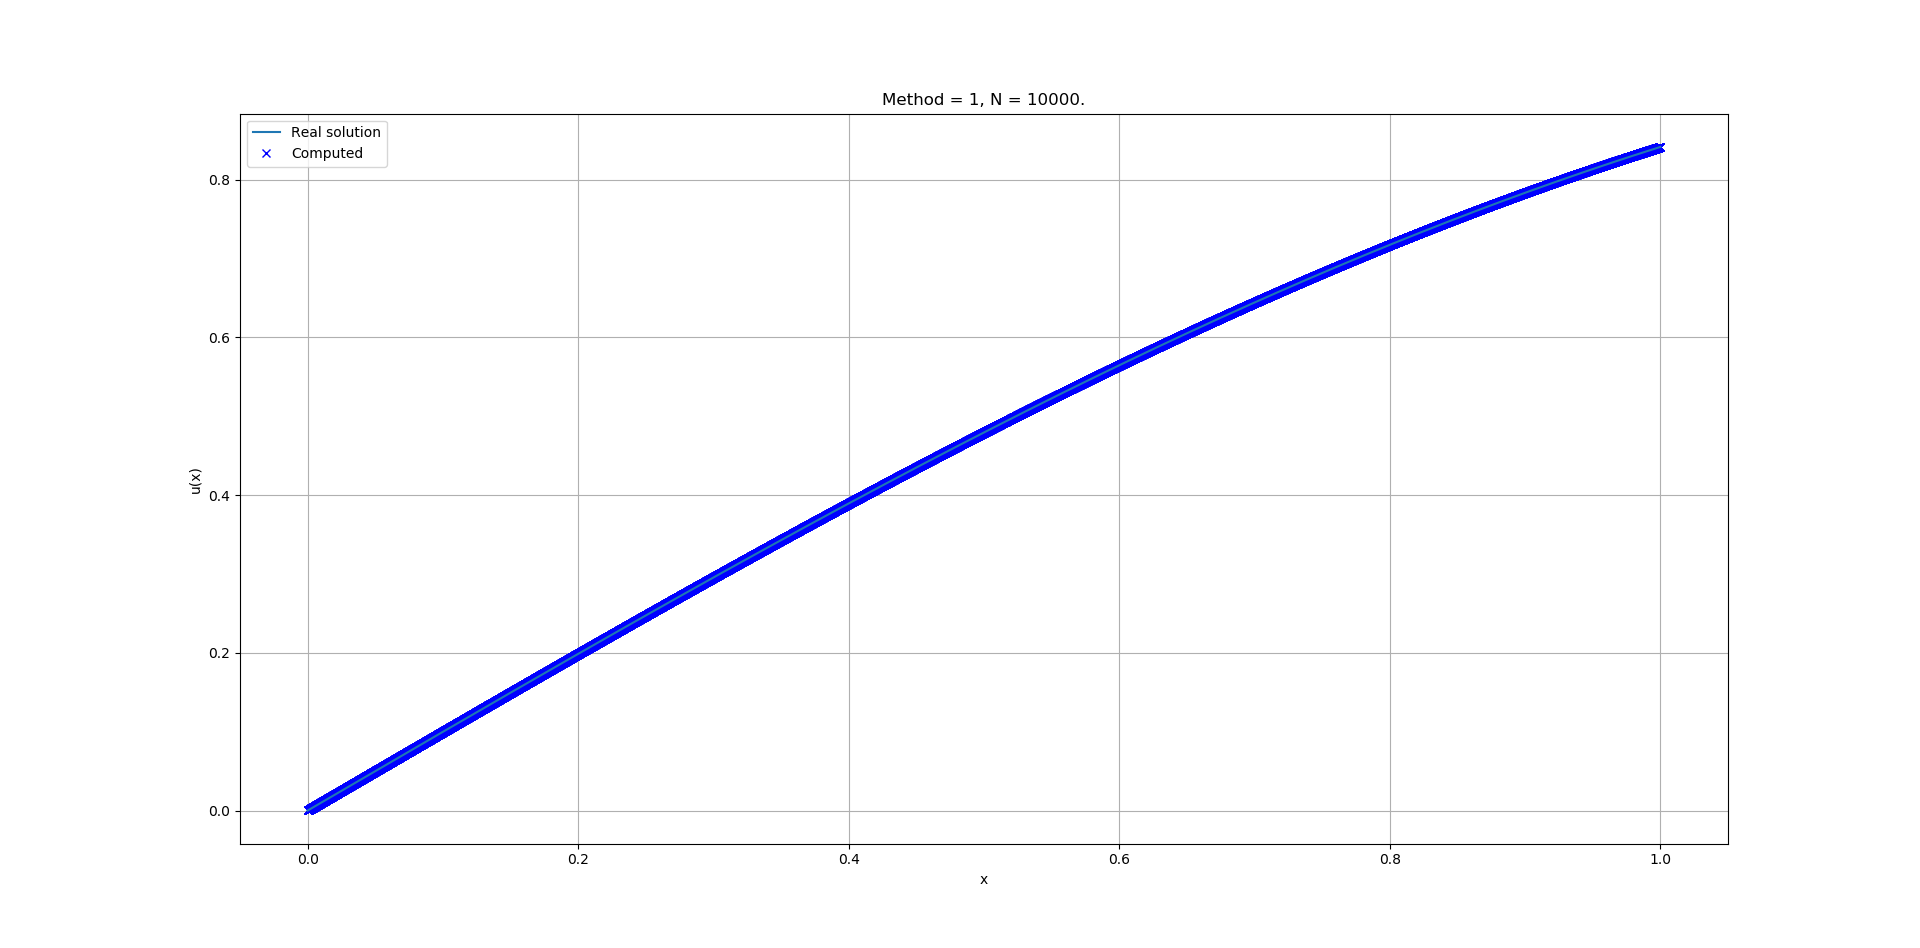
\includegraphics[width=14cm]{Figures/n10000.png}
  \caption{Computed solution}\label{fig:n10000}
\end{figure}




    


\clearpage

\section{Appendix}

\lstinputlisting[language=Python]{OneDimensional.py}













\end{CJK*}

\end{document}
